\documentclass[11pt]{article}

% ---------- layout ----------
\usepackage[margin=1.9cm,top=1.6cm,bottom=1.8cm]{geometry}
\usepackage[T1]{fontenc}
\usepackage[utf8]{inputenc}
\usepackage{mathpazo}           % warm serif body, no external font files needed
\usepackage{helvet}
\usepackage[table]{xcolor}      % [table] enables \rowcolor, used in Section 3
\usepackage{enumitem}
\usepackage{tikz}
\usetikzlibrary{arrows.meta,positioning}
\usepackage{array}
\usepackage{titlesec}
\usepackage{hyperref}
\usepackage{parskip}
\usepackage{tabularx}

% ---------- brand colours (matches the live prototype's palette) ----------
\definecolor{teal}{HTML}{1F6F5C}
\definecolor{tealdeep}{HTML}{123B32}
\definecolor{tealtint}{HTML}{DCEFE8}
\definecolor{coral}{HTML}{E2532D}
\definecolor{coraldeep}{HTML}{B33E1F}
\definecolor{inksoft}{HTML}{425146}
\definecolor{muted}{HTML}{71806F}
\definecolor{linecol}{HTML}{E3E1D2}

\hypersetup{colorlinks=true, linkcolor=teal, urlcolor=teal}

\titleformat{\section}
  {\normalfont\sffamily\bfseries\large\color{tealdeep}}
  {\thesection}{0.5em}{}
\titlespacing*{\section}{0pt}{10pt}{5pt}
\renewcommand{\thesection}{\textcolor{coral}{0\arabic{section}}}

\setlist[itemize]{leftmargin=1.3em, itemsep=1pt, topsep=2pt, parsep=0pt}
\setlist[enumerate]{leftmargin=1.5em, itemsep=1pt, topsep=2pt, parsep=0pt}

\newcommand{\keyline}[2]{{\sffamily\bfseries\footnotesize\color{inksoft}#1\ }#2}

\pagestyle{empty}

\begin{document}

% ---------- header ----------
\begin{center}
  {\sffamily\bfseries\Large\color{tealdeep} Practo for Animals --- Product \& Technology Concept}\\[2pt]
  {\sffamily\footnotesize\color{muted} Product \& Technology Intern Screening Assignment \quad\textbar\quad Submitted by Aman Sheikh}
\end{center}
\vspace{2pt}
\hrule height 1.4pt \color{coral}
\vspace{6pt}

% ============================================================
\section{Product Concept}

\keyline{Who:}{pet parents in urban India (primary); street-animal rescuers and feeders (secondary); vets, clinics, ambulances, NGOs and boarding facilities as the supply side.}

\keyline{First problem:}{in a crisis --- an injured stray, a sick pet after hours --- there is no reliable way to find a nearby, \emph{verified} vet, ambulance or rescuer. Information is scattered across Google, Instagram and WhatsApp groups. Discovery-in-a-crisis is the highest-intent, most frequent pain point, so it comes before routine browsing or booking.}

\keyline{Five MVP features:}{}
\begin{enumerate}
  \item \textbf{Location-based directory} of vets, ambulances, NGOs, rescuers and boarding facilities, filterable by distance and open-now status.
  \item \textbf{Verified provider profiles} --- timings, services offered, one-tap call/WhatsApp.
  \item \textbf{Emergency SOS mode} --- nearest 24$\times$7 vet, ambulance or rescuer, ranked by ETA and verification, not ads.
  \item \textbf{Pet health profile} --- basic pet details plus vaccination and visit history.
  \item \textbf{AI document upload} --- a photo of a prescription or report becomes a structured timeline entry with reminders.
\end{enumerate}

% ============================================================
\section{User Flow \& Prototype}

\textit{Home/Search $\rightarrow$ Results $\rightarrow$ Provider Profile $\rightarrow$ Call/WhatsApp, with a parallel emergency path: Home $\rightarrow$ SOS $\rightarrow$ Ranked nearby help $\rightarrow$ Call.}

\begin{center}
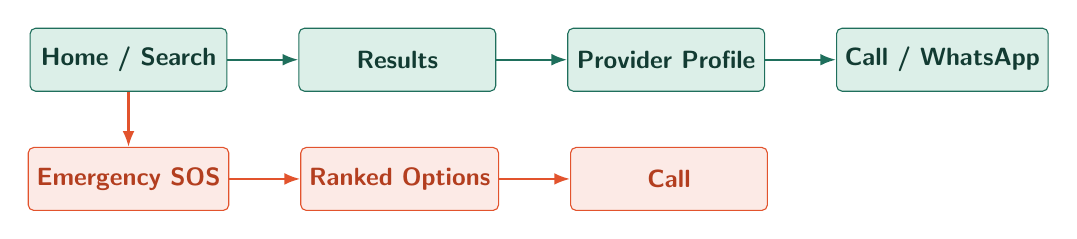
\begin{tikzpicture}[
    node distance=6mm and 9mm,
    box/.style={rectangle, rounded corners=2pt, draw=teal, fill=tealtint, text=tealdeep,
                font=\sffamily\bfseries\small, minimum height=8mm, minimum width=25mm, align=center, inner sep=3pt},
    sosbox/.style={box, draw=coral, fill=coral!12, text=coraldeep},
    arr/.style={-{Latex[length=2mm]}, teal, thick}
  ]
  \node[box] (home) {Home / Search};
  \node[box, right=of home] (results) {Results};
  \node[box, right=of results] (profile) {Provider Profile};
  \node[box, right=of profile] (contact) {Call / WhatsApp};

  \node[sosbox, below=7mm of home] (sos) {Emergency SOS};
  \node[sosbox, right=of sos] (ranked) {Ranked Options};
  \node[sosbox, right=of ranked] (call) {Call};

  \draw[arr] (home) -- (results);
  \draw[arr] (results) -- (profile);
  \draw[arr] (profile) -- (contact);
  \draw[arr, coral] (home) -- (sos);
  \draw[arr, coral] (sos) -- (ranked);
  \draw[arr, coral] (ranked) -- (call);
\end{tikzpicture}
\end{center}

\keyline{Prototype:}{7 working, clickable screens (Home, Search, Provider Profile, Emergency SOS, Pet Health Timeline, AI Document Upload, AI Symptom Triage) --- \url{https://pawzz-care.vercel.app} \textit{(placeholder --- final link added on deployment)}.}

% ============================================================
\section{AI \& Automation}

\begin{center}
\renewcommand{\arraystretch}{1.25}
\begin{tabularx}{\textwidth}{@{}>{\sffamily\bfseries\small}p{3.6cm} >{\small}X >{\small}X@{}}
\rowcolor{tealtint}
\textcolor{tealdeep}{Workflow} & \textcolor{tealdeep}{\sffamily\bfseries Processes} & \textcolor{tealdeep}{\sffamily\bfseries Automates} \\
Medical-document extraction & Photo of a prescription, vaccination card or lab report & Manually re-typing medical history into a record \\
Symptom triage \& routing & Free-text symptom description + species/age & Deciding urgent vs.\ routine and choosing where to route \\
Directory enrichment & Unstructured listings from Google, Instagram, WhatsApp & Structuring, de-duplicating and flagging bad entries \\
Rescue-story copy assistant & A rescuer's raw notes and photos & Drafting a publishable rescue story or fundraiser post \\
\end{tabularx}
\end{center}

\keyline{Own ideas:}{the emergency-first framing, ranking SOS results by ETA + verification (never ads), and using document-extraction to build a longitudinal pet health record are original to this concept. The base ``searchable directory'' pattern is inspired by Practo/JustDial-style platforms, as named in the brief.}

% ============================================================
\section{Technology}

\keyline{Stack:}{Next.js (mobile-responsive web) on Vercel; Supabase (Postgres + PostGIS, auth, file storage); Claude API for document extraction and triage chat.}

\keyline{Integrations:}{Google Maps/Places (location, geocoding) \textbullet\ WhatsApp Business API (contact, reminders) \textbullet\ Claude API (vision + text) \textbullet\ Razorpay (donations) \textbullet\ Firebase Cloud Messaging (push reminders).}

\keyline{Connections:}{Client $\rightarrow$ API layer $\rightarrow$ Postgres/PostGIS (providers, pets, records) + object storage (uploaded documents). The AI layer sits beside the API for extraction/triage; Maps, WhatsApp and Razorpay are called from the API layer as needed.}

% ============================================================
\section{MVP Thinking --- 30 Days}

\begin{center}
\renewcommand{\arraystretch}{1.15}
\begin{tabularx}{\textwidth}{@{}>{\small}X @{\hspace{10mm}} >{\small}X@{}}
{\sffamily\bfseries\color{tealdeep} Build} & {\sffamily\bfseries\color{muted} Leave out} \\
Directory + geo-search, provider profiles, SOS flow, manual pet profile, and the AI document-upload feature --- launched Gurgaon-only with 30--50 manually onboarded, verified listings. &
Booking \& payments, native mobile apps, self-serve provider onboarding, reviews/ratings, AI chat triage (needs tuning), multi-city expansion. \\
\end{tabularx}
\end{center}

\vspace{4pt}
\hrule height 0.6pt \color{linecol}
\vspace{4pt}
{\footnotesize\color{muted}
\textbf{\color{inksoft}Tools \& AI platforms used:} Claude (Claude Code) for product thinking, the working prototype, this document, and the extended web write-up. 
\newline
\quad
\textbf{\color{inksoft}Extended documentation:} \url{https://pawzz-care.vercel.app/case-study.html} \textit{(placeholder --- final link added on deployment)}.
}

\end{document}
